% Copyright 2004 by Till Tantau <tantau@users.sourceforge.net>.
%
% In principle, this file can be redistributed and/or modified under
% the terms of the GNU Public License, version 2.
%
% However, this file is supposed to be a template to be modified
% for your own needs. For this reason, if you use this file as a
% template and not specifically distribute it as part of a another
% package/program, I grant the extra permission to freely copy and
% modify this file as you see fit and even to delete this copyright
% notice. 

\documentclass{beamer}

\usepackage{blindtext}
\usepackage{tcolorbox}
\usepackage{soul}

\usepackage{amsmath}
\usepackage{amssymb}
\usepackage{amsthm}
\usepackage{amsfonts}

\makeatletter
\newcommand\xleftrightarrow[2][]{%
  \ext@arrow 9999{\longleftrightarrowfill@}{#1}{#2}}
\newcommand\longleftrightarrowfill@{%
  \arrowfill@\leftarrow\relbar\rightarrow}
\makeatother

\usefonttheme{professionalfonts} % using non standard fonts for beamer
\usefonttheme{serif} % default family is serif
%\usepackage{fontspec}
%\setmainfont{Liberation Serif}

% There are many different themes available for Beamer. A comprehensive
% list with examples is given here:
% http://deic.uab.es/~iblanes/beamer_gallery/index_by_theme.html
% You can uncomment the themes below if you would like to use a different
% one:
%\usetheme{AnnArbor}
%\usetheme{Antibes}
%\usetheme{Bergen}
%\usetheme{Berkeley}
%\usetheme{Berlin}
%\usetheme{Boadilla}
%\usetheme{boxes}
%\usetheme{CambridgeUS}
%\usetheme{Copenhagen}
%\usetheme{Darmstadt}
\usetheme{default}
%\usetheme{Frankfurt}
%\usetheme{Goettingen}
%\usetheme{Hannover}
%\usetheme{Ilmenau}
%\usetheme{JuanLesPins}
%\usetheme{Luebeck}
%\usetheme{Madrid}
%\usetheme{Malmoe}
%\usetheme{Marburg}
%\usetheme{Montpellier}
%\usetheme{PaloAlto}
%\usetheme{Pittsburgh}
%\usetheme{Rochester}
%\usetheme{Singapore}
%\usetheme{Szeged}
%\usetheme{Warsaw}



\title{Introduction to Signal Processing}

% A subtitle is optional and this may be deleted
\subtitle{Lecture 7: \textbf{Analysis of Continuous-time LTI Systems}}

\author{Sivakumar Balasubramanian}
% - Give the names in the same order as the appear in the paper.
% - Use the \inst{?} command only if the authors have different
%   affiliation.

\institute[Christian Medical College] % (optional, but mostly needed)
{
  \inst{}%
  Department of Bioengineering\\
  Christian Medical College, Bagayam\\
  Vellore 632002
}
% - Use the \inst command only if there are several affiliations.
% - Keep it simple, no one is interested in your street address.

\date{}
% - Either use conference name or its abbreviation.
% - Not really informative to the audience, more for people (including
%   yourself) who are reading the slides online

\subject{Lecture notes on signal processing}
% This is only inserted into the PDF information catalog. Can be left
% out.

% If you have a file called "university-logo-filename.xxx", where xxx
% is a graphic format that can be processed by latex or pdflatex,
% resp., then you can add a logo as follows:

% \pgfdeclareimage[height=0.5cm]{university-logo}{university-logo-filename}
% \logo{\pgfuseimage{university-logo}}

% Delete this, if you do not want the table of contents to pop up at
% the beginning of each subsection:
\AtBeginSubsection[]
{
  \begin{frame}<beamer>{Outline}
    \tableofcontents[currentsection,currentsubsection]
  \end{frame}
}

% Let's get started
\begin{document}
\setbeamertemplate{caption}{\raggedright\insertcaption\par}

\begin{frame}
  \titlepage
\end{frame}

% TRANSFER FUNCTIONS
\begin{frame}{Transfer Functions}

\begin{itemize}
\item LTI systems are described by linear constant coefficient differential equations,
\[ \sum_{i=0}^{N}a_i\frac{d^i}{dt^i}y(t) = \sum_{j=1}^{M}b_{j}\frac{d^j}{dt^j}x(t) \]
\item The transfer function is the ratio of the Laplace transform of $y(t)$ and $x(t)$ with zero initial conditions.
\[ H(s) = \frac{Y(s)}{X(s)} = \frac{\sum_{i=1}^{M}b_is^i}{\sum_{i=1}^{N}a_is^i} \]
where, $Y(s)$ and $X(s)$ are polynomials of $s$ with order $N$ and $M$, respectively, and the coefficients $a_i$ and $b_i$ are all real.
\item In practice, we only encounter transfer functions that are proper rational fractions,i.e. $N \geq M$.
\end{itemize}
\end{frame}

% Decomposition of transfer function
\begin{frame}{Decomposition of transfer functions}

\begin{itemize}
\item A transfer function $H(s)=\frac{P(s)}{Q(s)}$ can be  decomposed into two form, which are of practical importance: (a) \textit{pole-zero} representation and (b) \textit{partial fraction} representation.

\item \textbf{Pole-zero} representation: $P(s)$ and $Q(s)$ are factorized, yielding
\[ H(s) = \frac{\left(s-z_1\right)\left(s-z_2\right)\cdots\left(s-z_M\right)}{\left(s-p_1\right)\left(s-p_2\right)\cdots\left(s-p_M\right)} \]
where, $z_i,p_i \in \mathbb{C}$ are the zeros and poles of the transfer function, respectively.

\item \textbf{Partial fraction} representation: The following is the most general partial fraction representation,
\[ H(s) = R(s) + \sum_{i=1}^{N}\sum_{r=1}^{j_i}\frac{A_i}{\left(s-p_i\right)^r} \]
where, $p_i \in \mathbb{C}$ are the poles of the transfer function.
\end{itemize}
\end{frame}

% POLE-ZERO REPRESENTATION
\begin{frame}{Pole-Zero representation}
\[ H(s) = K\frac{\left(s-z_1\right)\left(s-z_2\right)\cdots\left(s-z_M\right)}{\left(s-p_1\right)\left(s-p_2\right)\cdots\left(s-p_M\right)} \]

\begin{itemize}
\item Here, the transfer function is decomposed into a product of simpler transfer functions.
\item The poles and zeros are real, or when they are complex, they occur in conjugate pairs (why?).
\item So, in effect any $H(s)$ of practical interest can be split into first and second order systems,
\[ G_1(s) = \frac{s + a}{s + b} \,\,\,\,\,\,\,\,\,\, G_2(s) = \frac{a_2s^2+a_1s+a_0}{b_2s^2+b_1s+b_0} \]
\end{itemize}
\begin{figure}
\centering
\caption{\tiny{Cascading of simpler systems ($1^{st}$ and $2^{nd}$ systems)}}
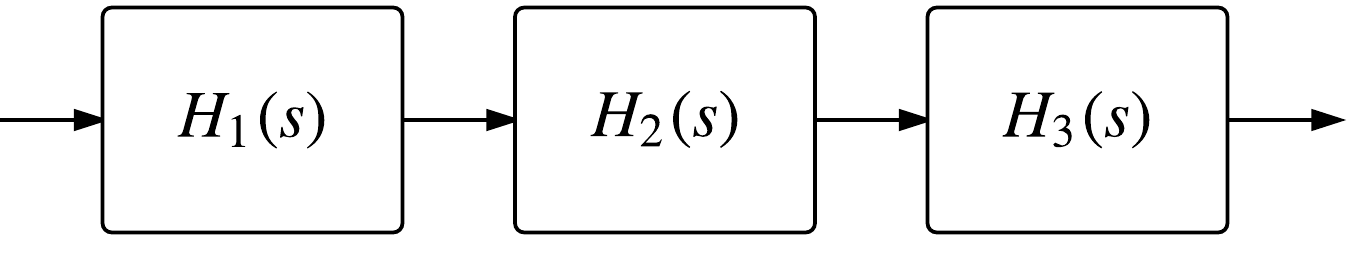
\includegraphics[width=0.6\textwidth]{img/series.png}
\end{figure}

\end{frame}

% POLE-ZERO REPRESENTATION
\begin{frame}{Pole-Zero representation}
\[ H(s) = K\frac{\left(s-z_1\right)\left(s-z_2\right)\cdots\left(s-z_M\right)}{\left(s-p_1\right)\left(s-p_2\right)\cdots\left(s-p_M\right)} \]

\begin{itemize}
\item The number of poles represent the number of memory elements in the system.
\item The poles can tell us about the stability of the system. Let $H(s) = \frac{1}{s+a}$. Answer the following quesitons about this system:
\begin{enumerate}
\item Where is the pole of the system?
\item If the system is causal, what is the ROC? What is the ROC when the system is anti-causal?
\item For a causal system, for what values of $a$ is the system stable?
\end{enumerate} 

Answering, these questions will help you understand the how the poles of a transfer function immediately tell us about the stability of a system. 
\end{itemize}
\end{frame}

% PARTIAL FRACTION REPRESENTATION
\begin{frame}{Partial Fraction Representation}

\[ H(s) = R(s) + \sum_{i=1}^{N}\sum_{r=1}^{j_i}\frac{A_i}{\left(s-p_i\right)^r} \]

Here, $A_i, p_i \in \mathbb{C}$. In order to have real coefficients for realizing a system, the abov equation can be re-written as the following,
\[ H(s) = R(s) + \sum_{i=1}^{L}\sum_{r=1}^{j_i}\frac{A_i}{\left(s-p_i\right)^r} + \sum_{i=1}^{M}\sum_{r=1}^{k_i}\frac{B_is + C_i}{\left(s^2+b_is+c_i\right)^r}\]

where, $A_i, B_i, C_i, p_i, b_i, c_i \in \mathbb{R}$, and $b_i^2-4c_i < 0$. 

For a proper rational function, where the order of the numerator is less than the order of the denominator, $R(s) = 0$.

\vspace{2mm}
How does one find out the $A_i$s, $B_i$s and $C_i$s?
\vspace{2mm}

\textbf{Examples:} Find the partial fraction representation for: (a) $\frac{s+3}{s^2+3s+5}$; (b) $\frac{s^3+5s^2+10s+3}{s^2+3s+5}$; and (c) $\frac{1}{s^3+s^2+2s+1}$.
\end{frame}

% PARTIAL FRACTION REPRESENTATION
\begin{frame}{Partial Fraction Representation}

\begin{itemize}
\item Using a partial fraction representation one can implement a transfer fucntion as a parallel combination of simpler ($1^{st}$ and $2^{nd}$ systems).
\end{itemize}
\vspace{-8mm}
\begin{figure}
\centering
\caption{\tiny{Parallel implementation of a system.}}
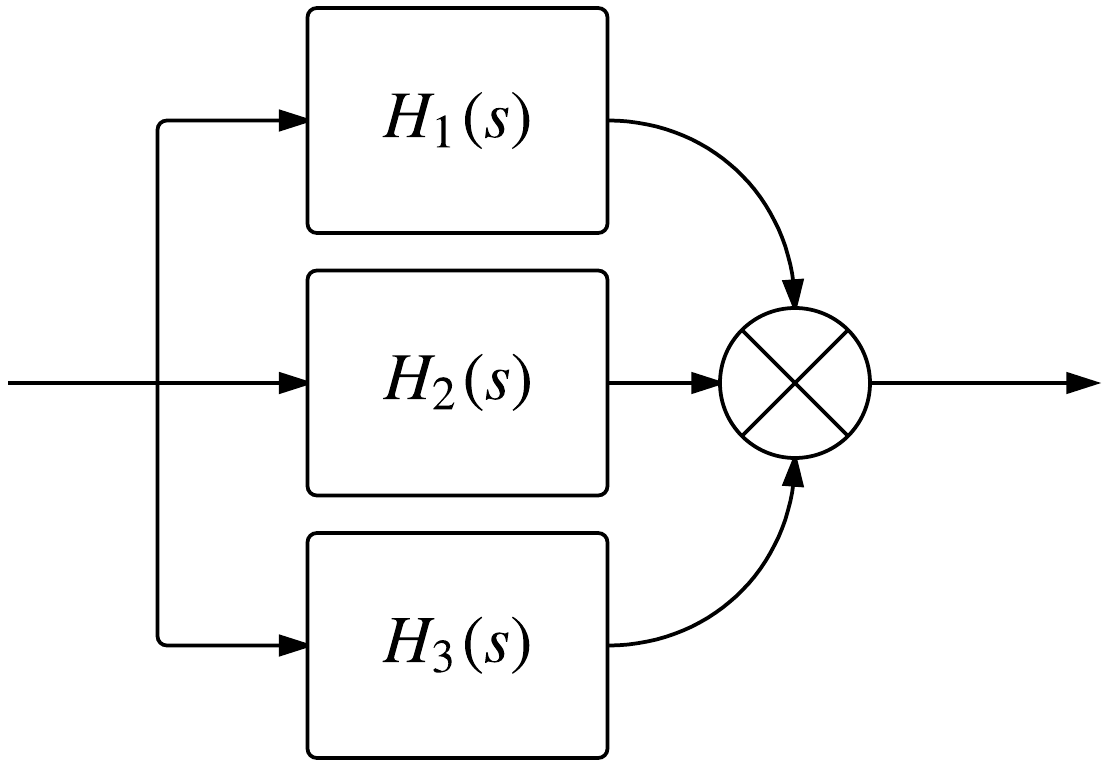
\includegraphics[width=0.7\textwidth]{img/parallel.png}
\end{figure}
\end{frame}

% FREQUENCY RESPONSE
\begin{frame}{Frequency Response}

The frequency response of a LTI system can be obtained from its transfer function.
\[ H(\omega) = H(s)\Big|_{s=j\omega} \]

For a causal and stable system, the poles of the system must lie in the left half of the $j\omega$ axis. This means that the ROC includes the $j\omega$ axis, and thus implies that the $H(j\omega)$ exists.

\textbf{Example}:
\[ H(s) = \frac{1}{s+a} \implies H(\omega) = \frac{1}{j\omega + a} \]
\[ H(s) = \frac{s+b}{s^2+cs+d} \implies H(\omega) = \frac{j\omega+b}{d - \omega^2 + j\omega d} \]

\end{frame}

% GEOMETRIC ESTIMATION OF FREQUENCY RESPONSE
\begin{frame}{Geometric estimation of frequency response.}

\[ H(s) = K\frac{\left(s - z_1\right)\left(s - z_2\right)\cdots\left(s - z_M\right)}{\left(s - p_1\right)\left(s - p_2\right)\cdots\left(s - p_N\right)}\]

\[\implies H(\omega) = K\frac{\left(j\omega - z_1\right)\left(j\omega - z_2\right)\cdots\left(j\omega - z_M\right)}{\left(j\omega - p_1\right)\left(j\omega - p_2\right)\cdots\left(j\omega - p_N\right)} \]

Here, the magnitude and phase responses can be estimated as the product and the sum of the contributions from the poles and the zeros.
\[ \text{Magnitude Response} =\left|H(\omega)\right| = K \frac{\Pi_{i=1}^{M}\left|j\omega - z_i\right|}{\Pi_{i=1}^{N}\left|j\omega - p_i\right|} \]
\[ \text{Phase Response} = \angle H(\omega) =  \sum_{i=1}^{M}\angle \left(j\omega - z_i\right) - \sum_{i=1}^{N}\angle \left(j\omega - p_i\right) \]

\end{frame}

% GEOMETRIC ESTIMATION OF FREQUENCY RESPONSE
\begin{frame}{Geometric estimation of frequency response.}
\vspace{-5mm}
\begin{figure}
\centering
\caption{\tiny{The following figure demonstrates how to determine the frequency response geometrically.}}
\vspace{-1mm}
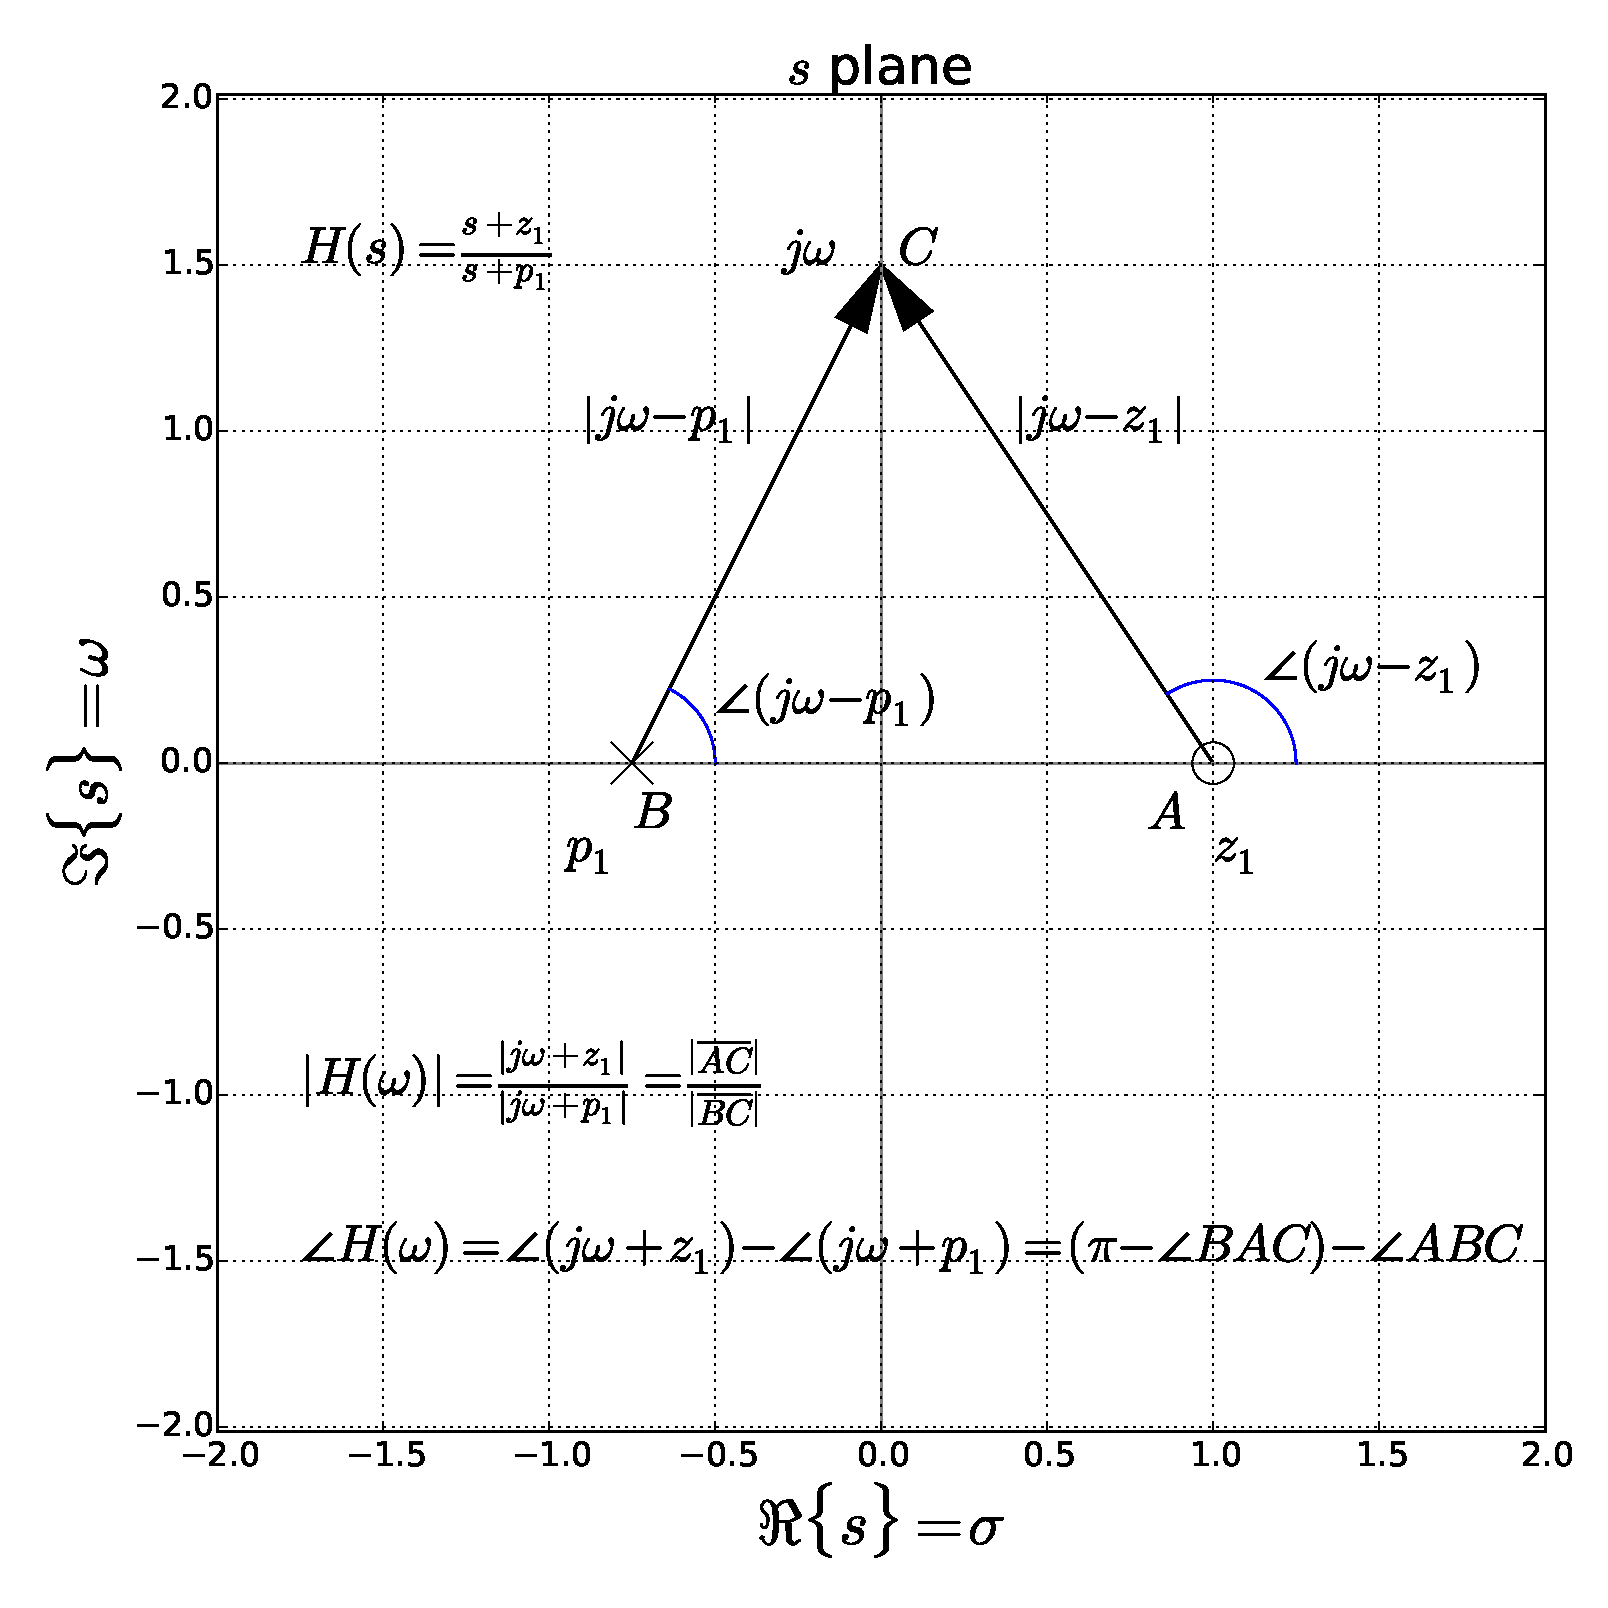
\includegraphics[width=0.76\textwidth]{img/geo_freq_resp.eps}
\end{figure}

\end{frame}

% FREQUENCY RESPONSE OF 1ST ORDER SYSTEMS
\begin{frame}{Frequency response of 1$^{st}$ order system}
Consider a $1^{st}$ order system, $ H(s) = \frac{p}{s+p} $

\small{The plot of the magnitude and phase responses are shown in the following figure. \textbf{Verify using the geometric method that these responses are correct.}}
\vspace{-2mm}
\begin{figure}
\centering
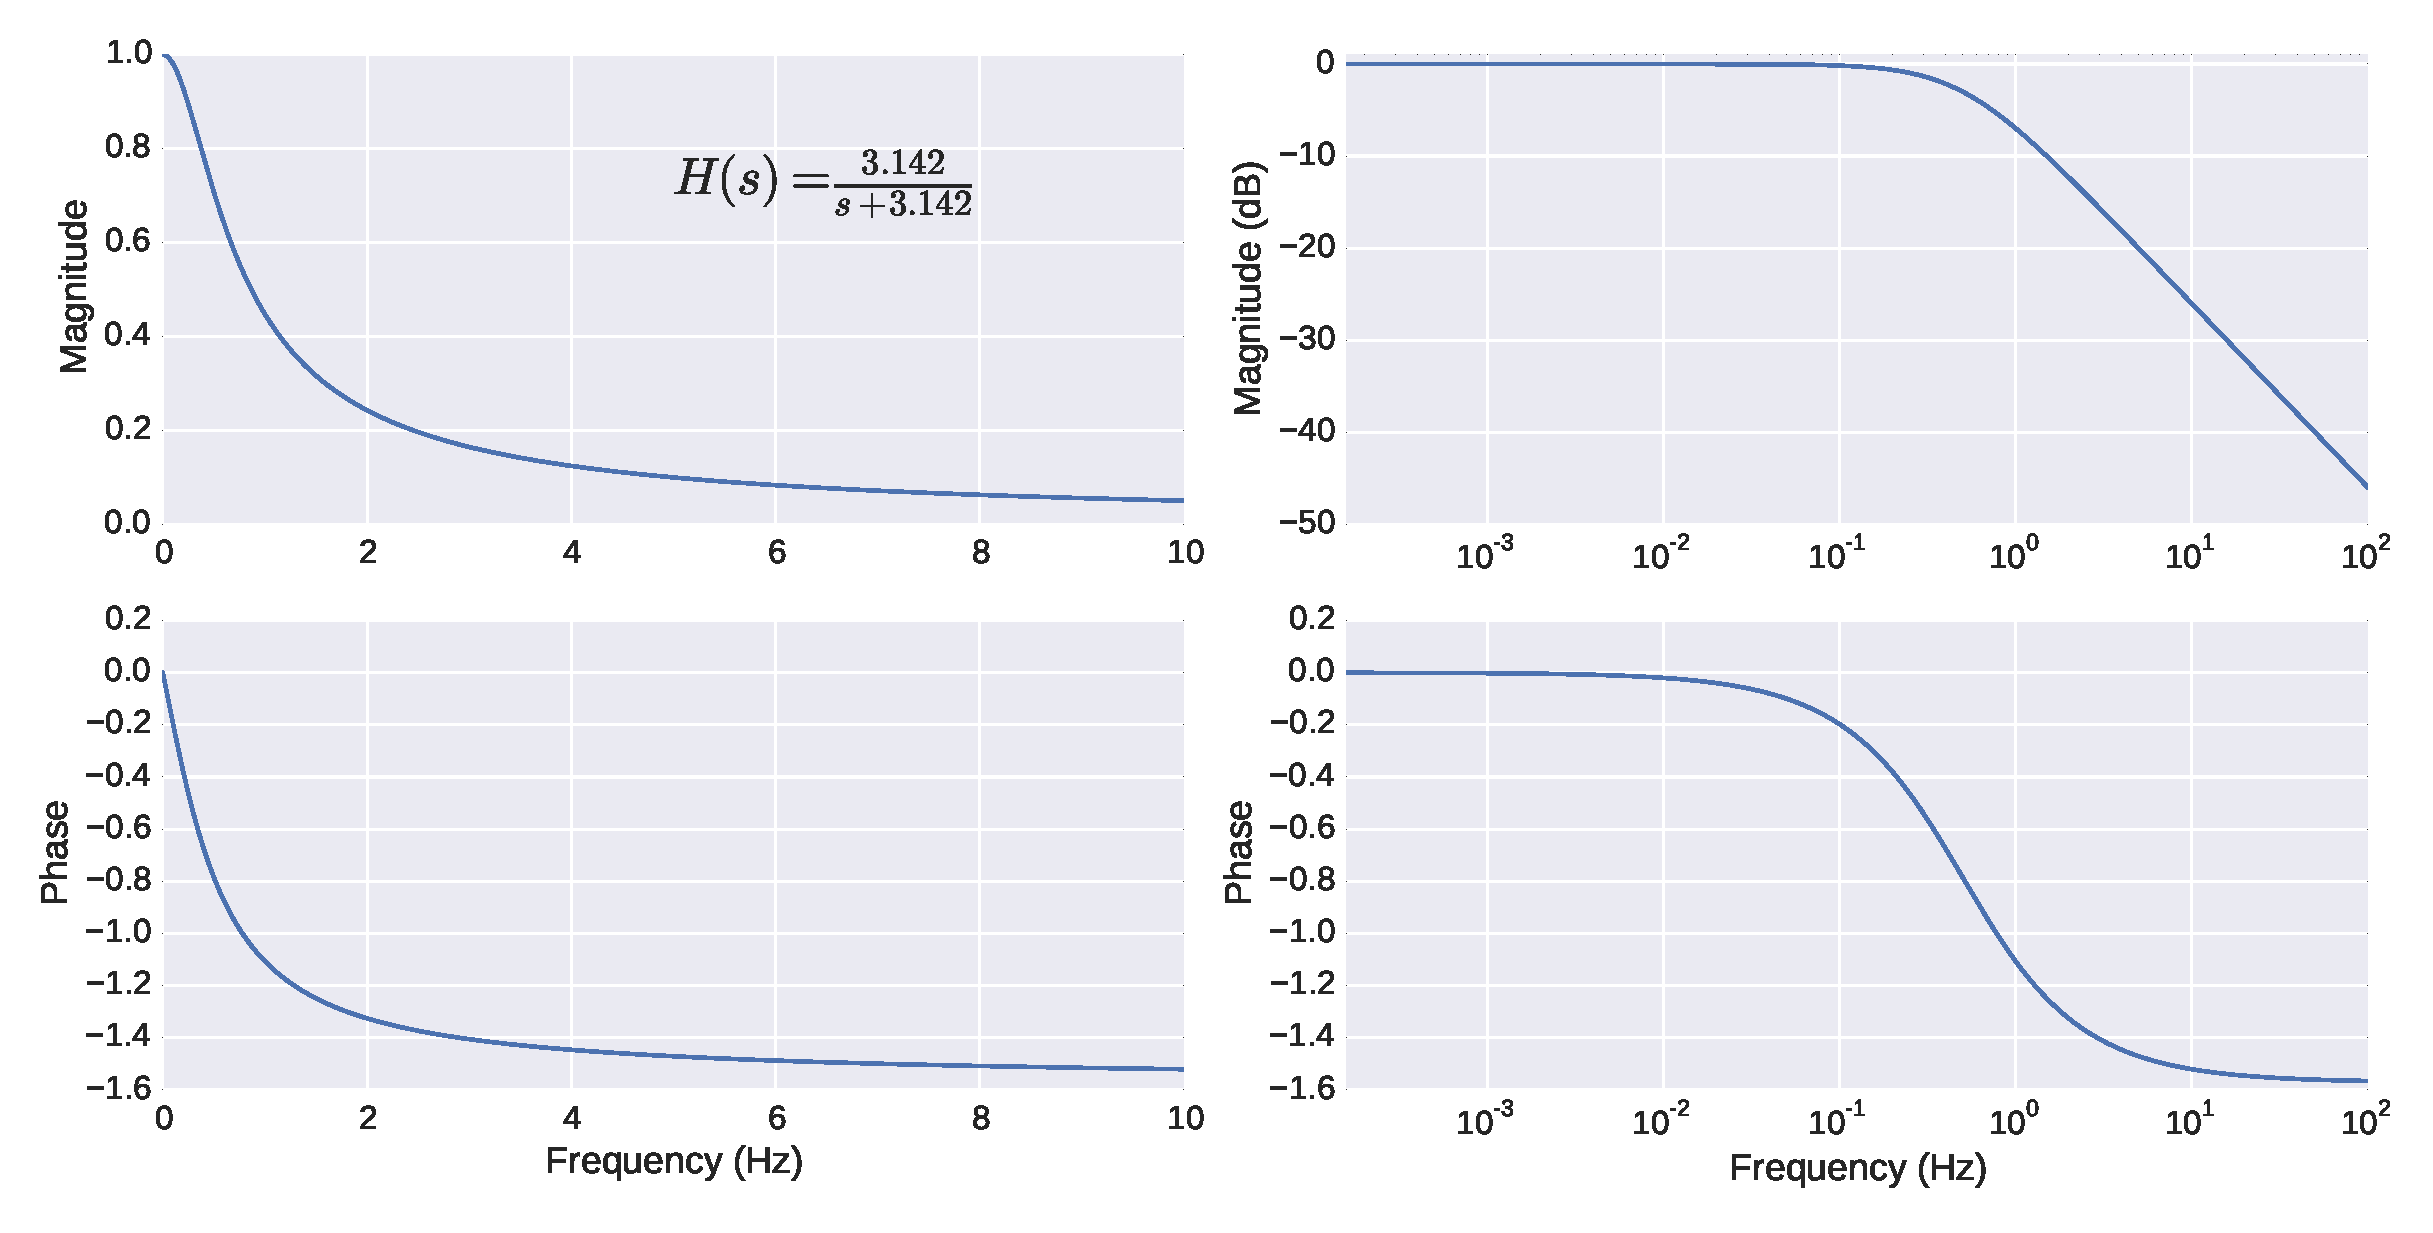
\includegraphics[width=\textwidth]{img/1st_sys.eps}
\end{figure}
\vspace{-4mm}
\small{The right column shown the magnitude and phase responses in with a logarithmic $x$ axis. Note that in the top-right plot the magnitude is presented in \textit{decibels}, i.e. $20\log \left|H(\omega)\right|$.}
\end{frame}

% FREQUENCY RESPONSE OF 2ND ORDER SYSTEMS
\begin{frame}{Frequency response of 2$^{nd}$ order system}
\begin{small}
Consider a $2^{nd}$ order system, $ H(s) = \frac{a_0}{s^2+a_1s+a_0} $. This transfer function can be characterized in three different ways:
\begin{enumerate}
\item By the parameters, $a_0$ and $a_1$.
\item By the real and imaginary values of the poles, $\Re\{p_1\}$, $\Re\{p_2\}$, $\Im\{p_1\}$,  and $\Im\{p_2\}$. $ H(s) = \frac{a_0}{(s - p_1)(s-p_2)} $
\item By the resonant frequency $\omega_n$ and the quality factor $Q$. $ H(s) = \frac{\omega_n^2}{s^2+(\omega_n/Q)s +\omega_n^2} $
\end{enumerate}
$Q=\left|\frac{H(\omega_n)}{H(0)}\right|$ is the ratio of the magnitude at $\omega=\omega_n$ with respect to that of $\omega=0$. It is also approximately equal to the ratio of the resonant frequency and the 3dB bandwidth around the resonant frequency $Q=\frac{\omega_n}{\Delta \omega_{3dB}}$. And also,
\[ \frac{\Im\{p_1\}}{\Re\{p_1\}} = \sqrt{4Q^2-1} \]
\textbf{What is the locus of all pole locations on the s plane with the same Q factor?}
\end{small}
\end{frame}

% FREQUENCY RESPONSE OF 2ND ORDER SYSTEMS
\begin{frame}{Frequency response of 2$^{nd}$ order system}
Consider a $2^{nd}$ order system, $ H(s) = \frac{\omega_n^2}{s^2+(\omega_n/Q)s+\omega_n^2} $

\small{The plot of the magnitude and phase responses are shown in the following figure. \textbf{Verify using the geometric method that these responses are correct.}}
\vspace{-2mm}
\begin{figure}
\centering
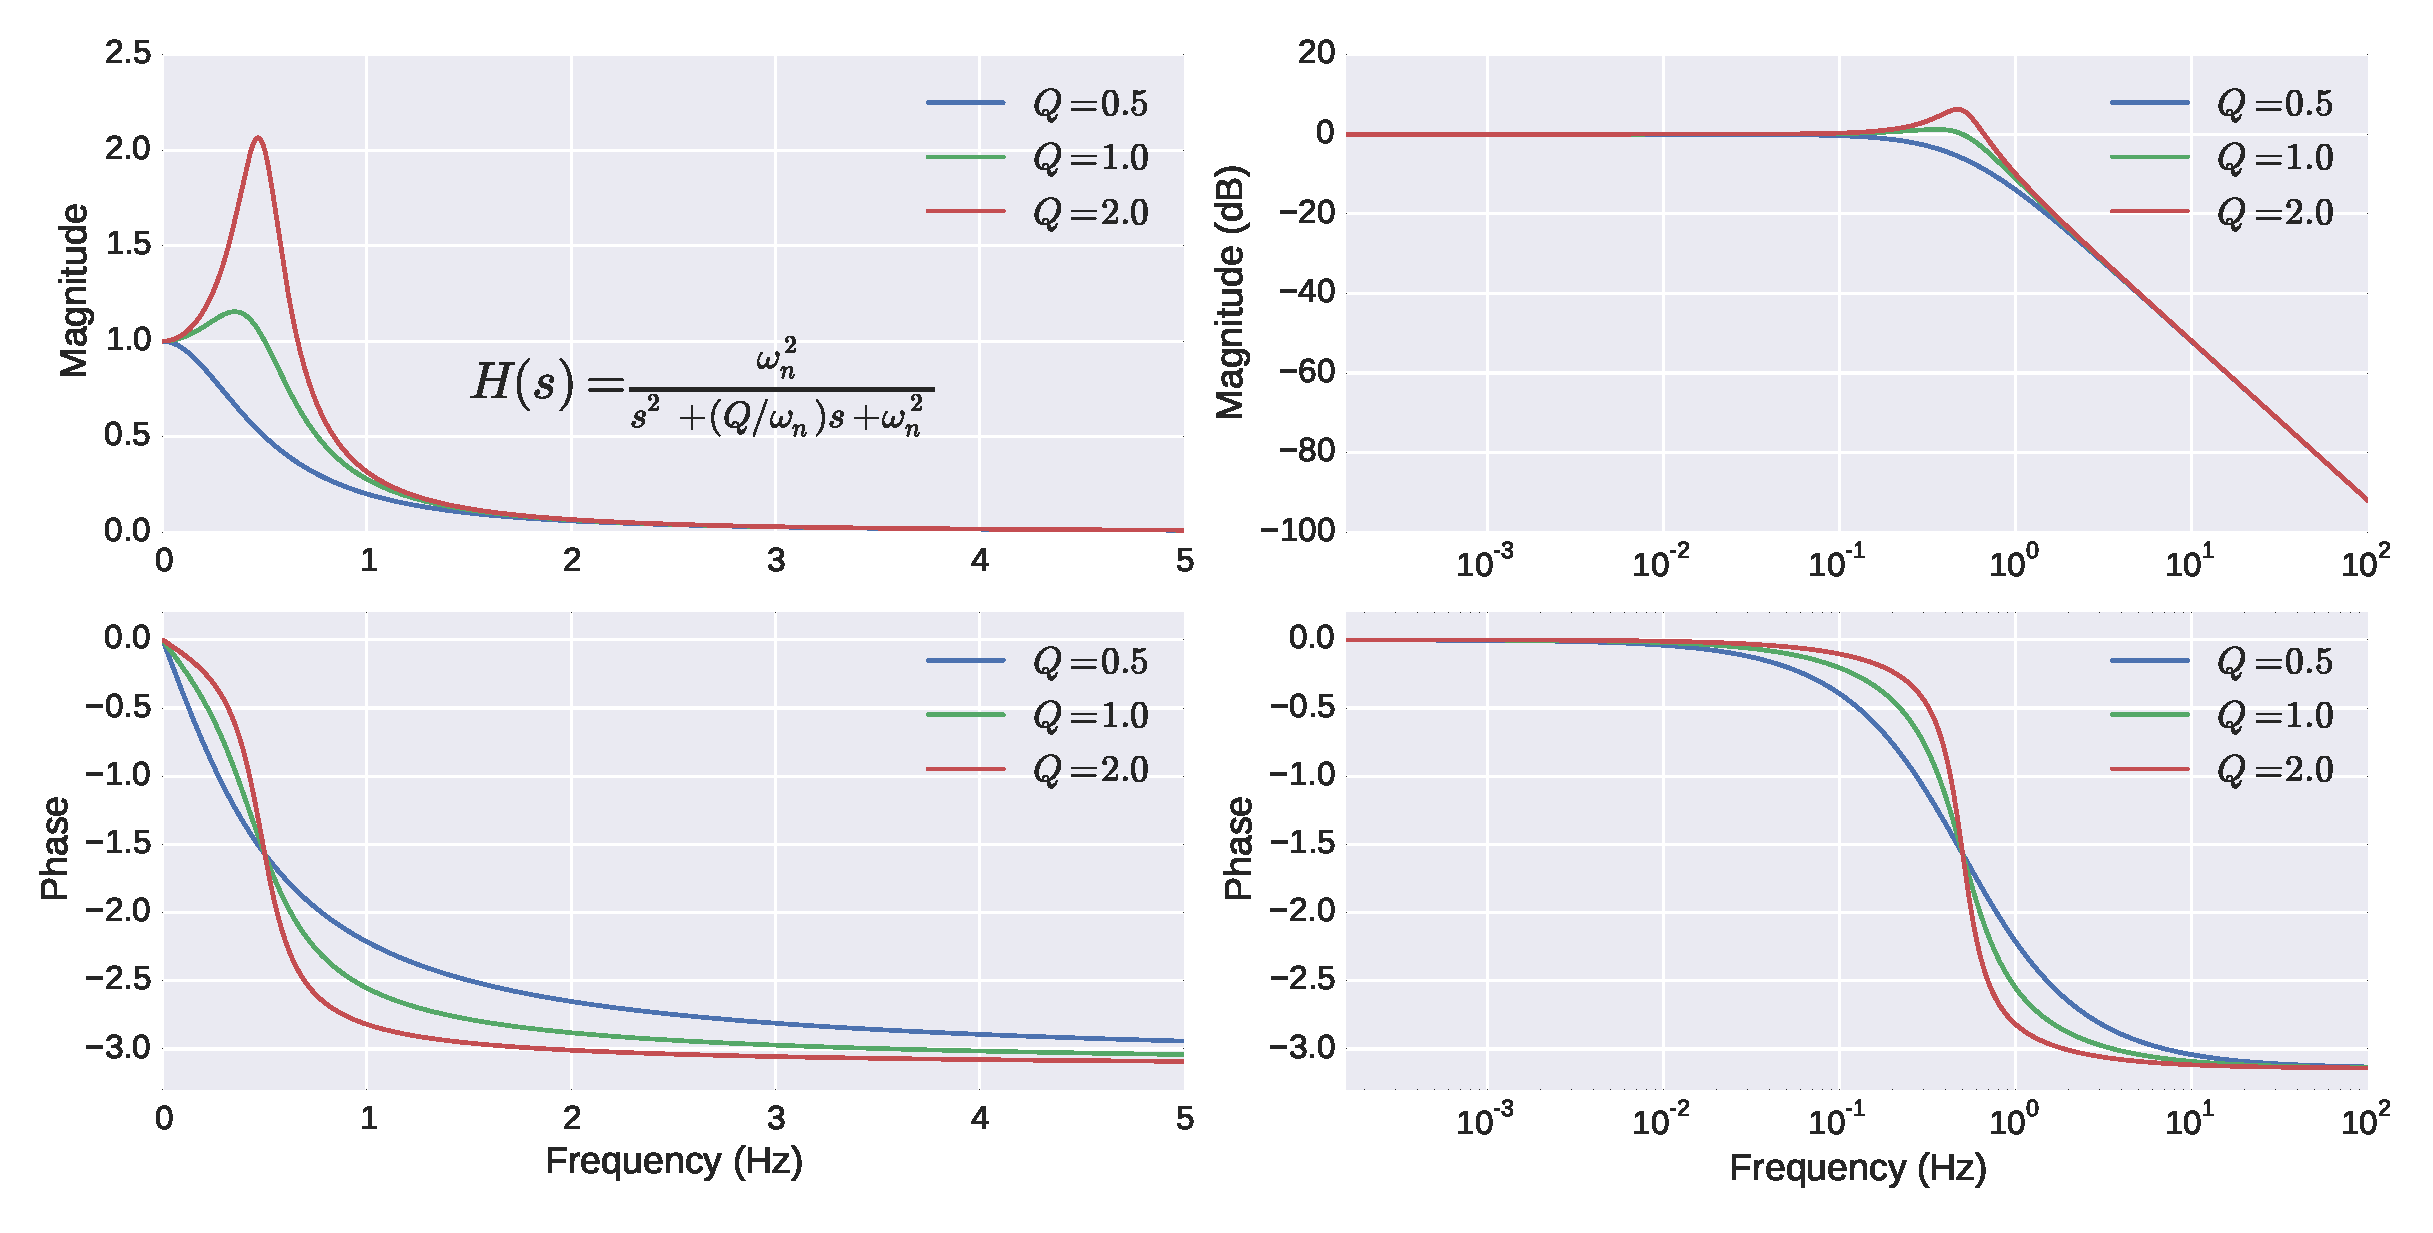
\includegraphics[width=\textwidth]{img/2nd_sys.eps}
\end{figure}
\end{frame}

% BODE PLOTS
\begin{frame}{Bode plots}

\begin{itemize}
\item Bode plots provide a manual method to quickly sketch approximate magnitude and phase responses.
\item Bode plots are asymptotic approximations of the actual magnitude and phase responses.
\item Both the magnitude and phase plots are plotted on a logarithmic frequency axis.
\item Magnitude is represented in \textit{decibels}. The use of the decibel scale, will make the product of the different zeros and poles into a summation.
\begin{small}
\[ \text{Magnitude Response} =\left|H(\omega)\right| = K \frac{\Pi_{i=1}^{M}\left|j\omega - z_i\right|}{\Pi_{i=1}^{N}\left|j\omega - p_i\right|} \]
\[ \text{Magnitude Response (in dB)} = 20\log \left|H(\omega)\right| \]
\[ = 20 \log K + \sum_{i=1}^{M}20\log\left|j\omega - z_i\right| - \sum_{i=1}^{N}20\log\left|j\omega - p_i\right| \]
\end{small}
\end{itemize}

\end{frame}

% BODE PLOTS
\begin{frame}{Bode plots: Magnitude plot}

\begin{itemize}
\item To understand how to plot the magnitude response, we will look at two cases: (a) a system with a single real pole; and (b) a system with a single real zero.
\item System with a single real pole.
\[ H(\omega) = \frac{\omega_0}{j\omega + \omega_0} \implies \left|H(\omega)\right|_{dB}=20\log\left|\frac{\omega_0}{j\omega+\omega_0}\right|\]
\[ \left|H(\omega)\right|_{dB}=-20\log	\sqrt{1 + \left(\frac{\omega}{\omega_0}\right)^2} \approx \begin{cases}
0 & \omega \ll \omega_0\\
-20\log\left(\frac{\omega}{\omega_0}\right)& \omega \gg \omega_0
\end{cases} \]
\end{itemize}
This implies that for frequencies well below $\omega_0$, the magnitude is close to 0dB.

When the frequency is well above $\omega_0$, the magnitude decreases linearly as a log of the frequency. A 10 fold increase in $\frac{\omega}{\omega_0}$, will lead to -20dB reduction in the magnitude.

\end{frame}

% BODE PLOTS
\begin{frame}{Bode plots: Magnitude plot}

\begin{itemize}
\item System with a single real zero.
\[ H(\omega) = \frac{j\omega + \omega_0}{\omega_0} \implies \left|H(\omega)\right|_{dB}=20\log\left|\frac{j\omega+\omega_0}{\omega_0}\right|\]
\[ \left|H(\omega)\right|_{dB}=20\log\sqrt{1 + \left(\frac{\omega}{\omega_0}\right)^2} \approx \begin{cases}
0 & \omega \ll \omega_0\\
20\log\left(\frac{\omega}{\omega_0}\right)& \omega \gg \omega_0
\end{cases} \]
\end{itemize}
This implies that for frequencies well below $\omega_0$, the magnitude is close to 0dB.

When the frequency is well above $\omega_0$, the magnitude decreases linearly as a log of the frequency. A 10 fold increase in $\frac{\omega}{\omega_0}$, will lead to +20dB increase in the magnitude.

\end{frame}

% BODE PLOTS
\begin{frame}{Bode plots: Phase plot}
\begin{small}
We can do a similar approximation for the phase plot.
\begin{itemize}
\item System with a single real pole.
\[ H(\omega) = \frac{\omega_0}{j\omega + \omega_0} \implies \angle H(\omega)=-\arctan \left(\frac{\omega}{\omega_0}\right)\]
\[ \angle H(\omega) \approx \begin{cases}
0 & \omega < 0.1\omega_0\\
-\frac{\pi}{4} & \omega = \omega_0\\
-\frac{\pi}{2} & \omega > 10\omega_0 
\end{cases} \]
\item System with a single real zero.
\[ H(\omega) = \frac{j\omega + \omega_0}{\omega_0} \implies \angle H(\omega)=\arctan \left(\frac{\omega}{\omega_0}\right)\]
\[ \angle H(\omega) \approx \begin{cases}
0 & \omega < 0.1\omega_0\\
\frac{\pi}{4} & \omega = \omega_0\\
\frac{\pi}{2} & \omega > 10\omega_0 
\end{cases} \]
\end{itemize}
Between $0.1\omega_0$ and $10\omega_0$, we use a linear approximation as a function of the log of the frequency.
\end{small}
\end{frame}

% BODE PLOTS
\begin{frame}{Bode plots of first order pole and zero}
Frequency response and Bode approximations of systems with a first order pole and first order zero.
\begin{figure}
\centering
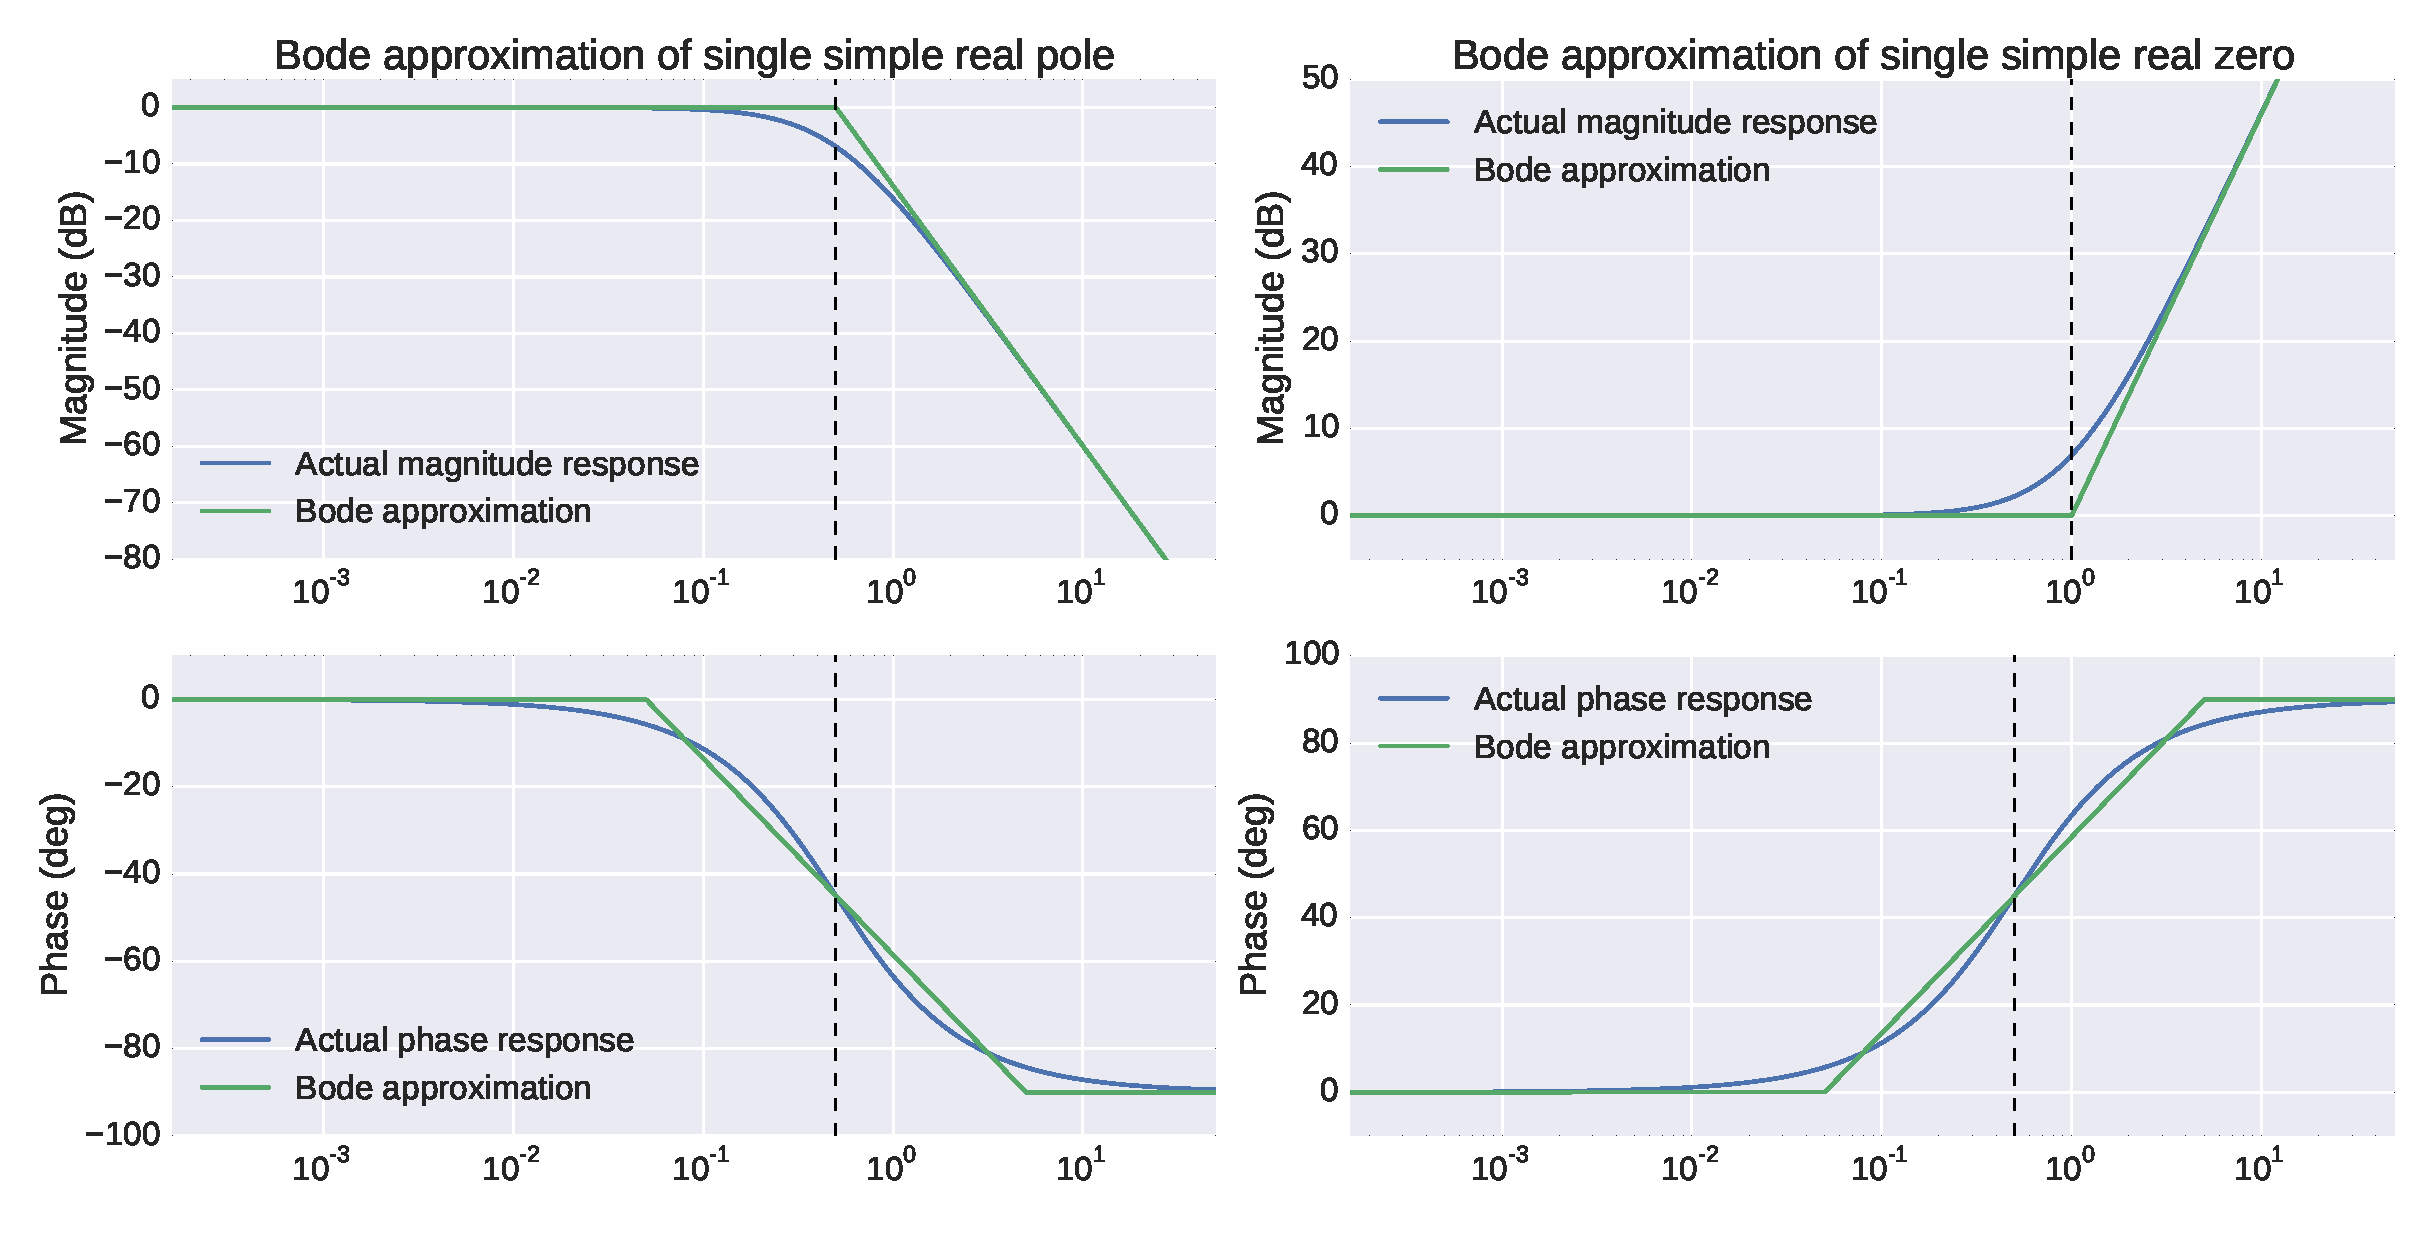
\includegraphics[width=1.05\textwidth]{img/1st_bode.eps}
\end{figure}
\end{frame}

% BODE PLOTS
\begin{frame}{Bode plots: Magnitude plot of $2^{nd}$ order system}
\begin{small}
System with $2^{nd}$ order poles
\[ H(\omega) = \frac{\omega_n^2}{\omega_n^2 - \omega^2 + j\omega\frac{\omega_n}{Q}}  \implies \left|H(\omega)\right|_{dB}=20\log\left|\frac{1}{1 - \left(\frac{\omega}{\omega_n}\right)^2 + j\frac{\omega/\omega_n}{Q}}\right|\]
\[ \left|H(\omega)\right|_{dB}=-20\log	\sqrt{\left(1 - \left(\frac{\omega}{\omega_n}\right)^2\right)^2 + \left(\frac{\omega/\omega_n}{Q}\right)^2} \]
\[ \left|H(\omega)\right|_{dB} \approx \begin{cases}
0 & \omega \ll \omega_0\\
-20 \log \left(\frac{1}{Q}\right) & \omega = \omega_0\\
-40\log\left(\frac{\omega}{\omega_0}\right)& \omega \gg \omega_0
\end{cases} \]

The Bode approximation works well for small and large $\omega$, but close to $\omega_0$, the approximation can be poor depending on the value of $Q$.

For the case of $2^{nd}$ order zeros, the signs of the magnitude response will need to reversed.
\end{small}
\end{frame}

% BODE PLOTS
\begin{frame}{Bode plots: Phase plot of $2^{nd}$ order system}
System with $2^{nd}$ order poles
\[ H(\omega) = \frac{\omega_n^2}{\omega_n^2 - \omega^2 + j\omega\frac{\omega_n}{Q}}  \implies \angle H(\omega)= -\arctan \left(\frac{\omega/\omega_nQ}{1-\left(\omega/\omega_n\right)^2}\right)\]
\[ \angle H(\omega) \approx \begin{cases}
0 & \omega \ll 0.1\omega_0\\
-\frac{\pi}{2} & \omega = \omega_0\\
-\pi & \omega \gg 10\omega_0
\end{cases} \]

For the case of $2^{nd}$ order zeros, the signs of the magnitude response will need to reversed.
\end{frame}

% BODE PLOTS
\begin{frame}{Bode plots of second order poles and zeros}
Frequency response and Bode approximations of systems with a $2^{nd}$ order poles and zeros.
\begin{figure}
\centering
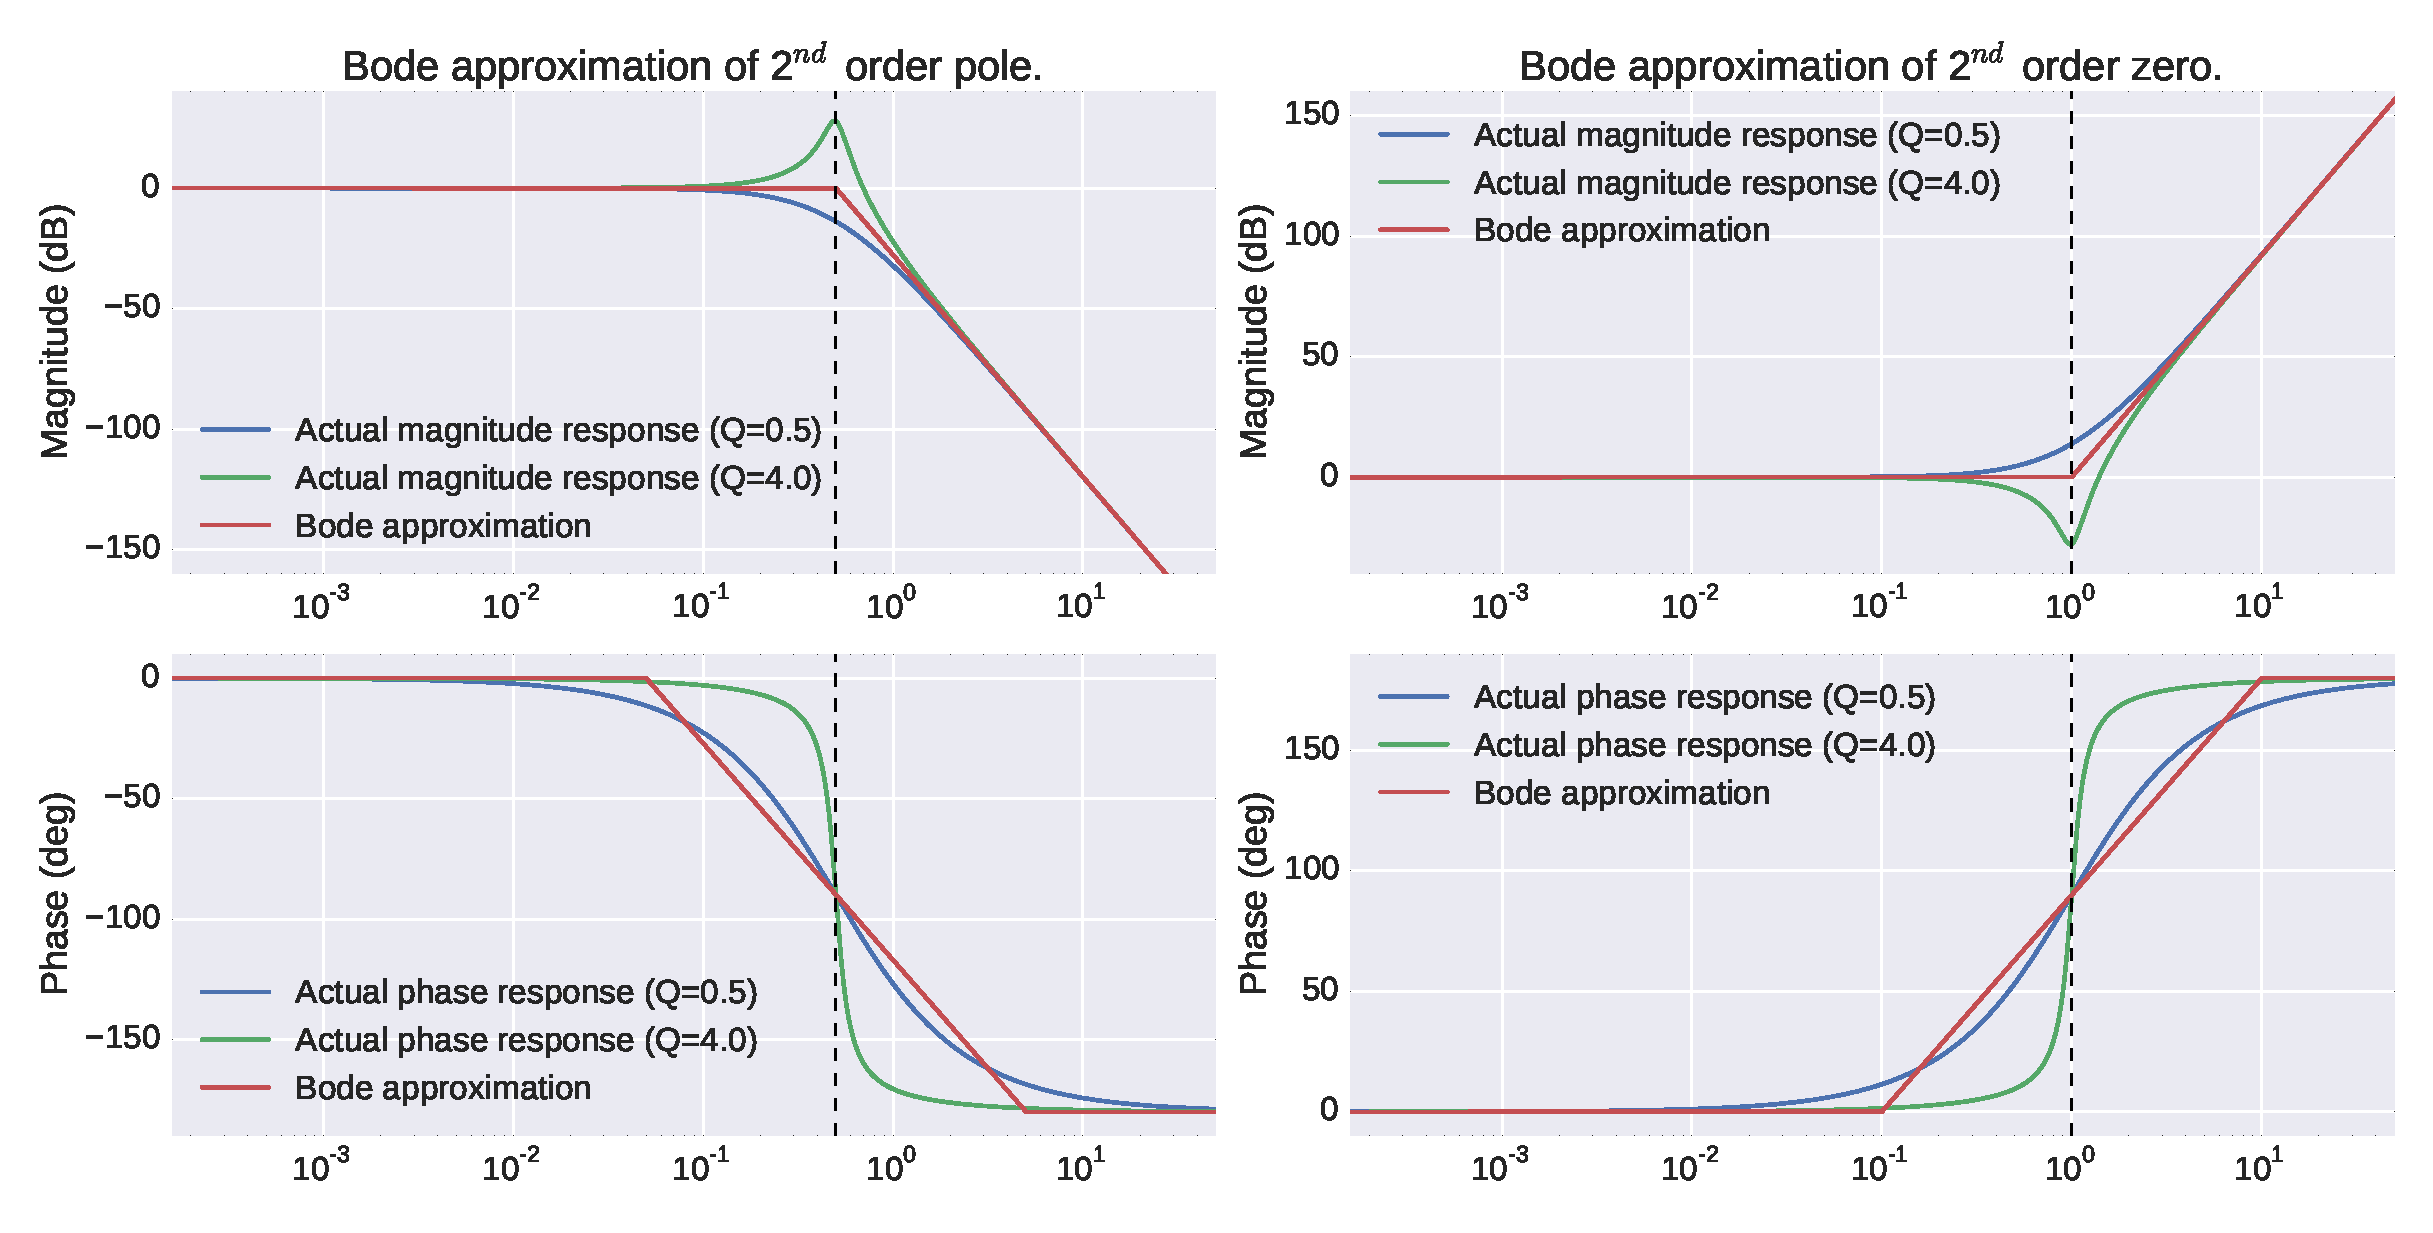
\includegraphics[width=1.05\textwidth]{img/2nd_bode.eps}
\end{figure}
\end{frame}

% BODE PLOT
\begin{frame}{Bode plot example}
Consider the following transfer function,
\[ H(s) = \frac{(s+100\pi)(s+2000\pi)(s+10000\pi)}{(s+20\pi)(s+1000\pi)(s+2000\pi)(s+15000\pi)} \]

\begin{figure}
\centering
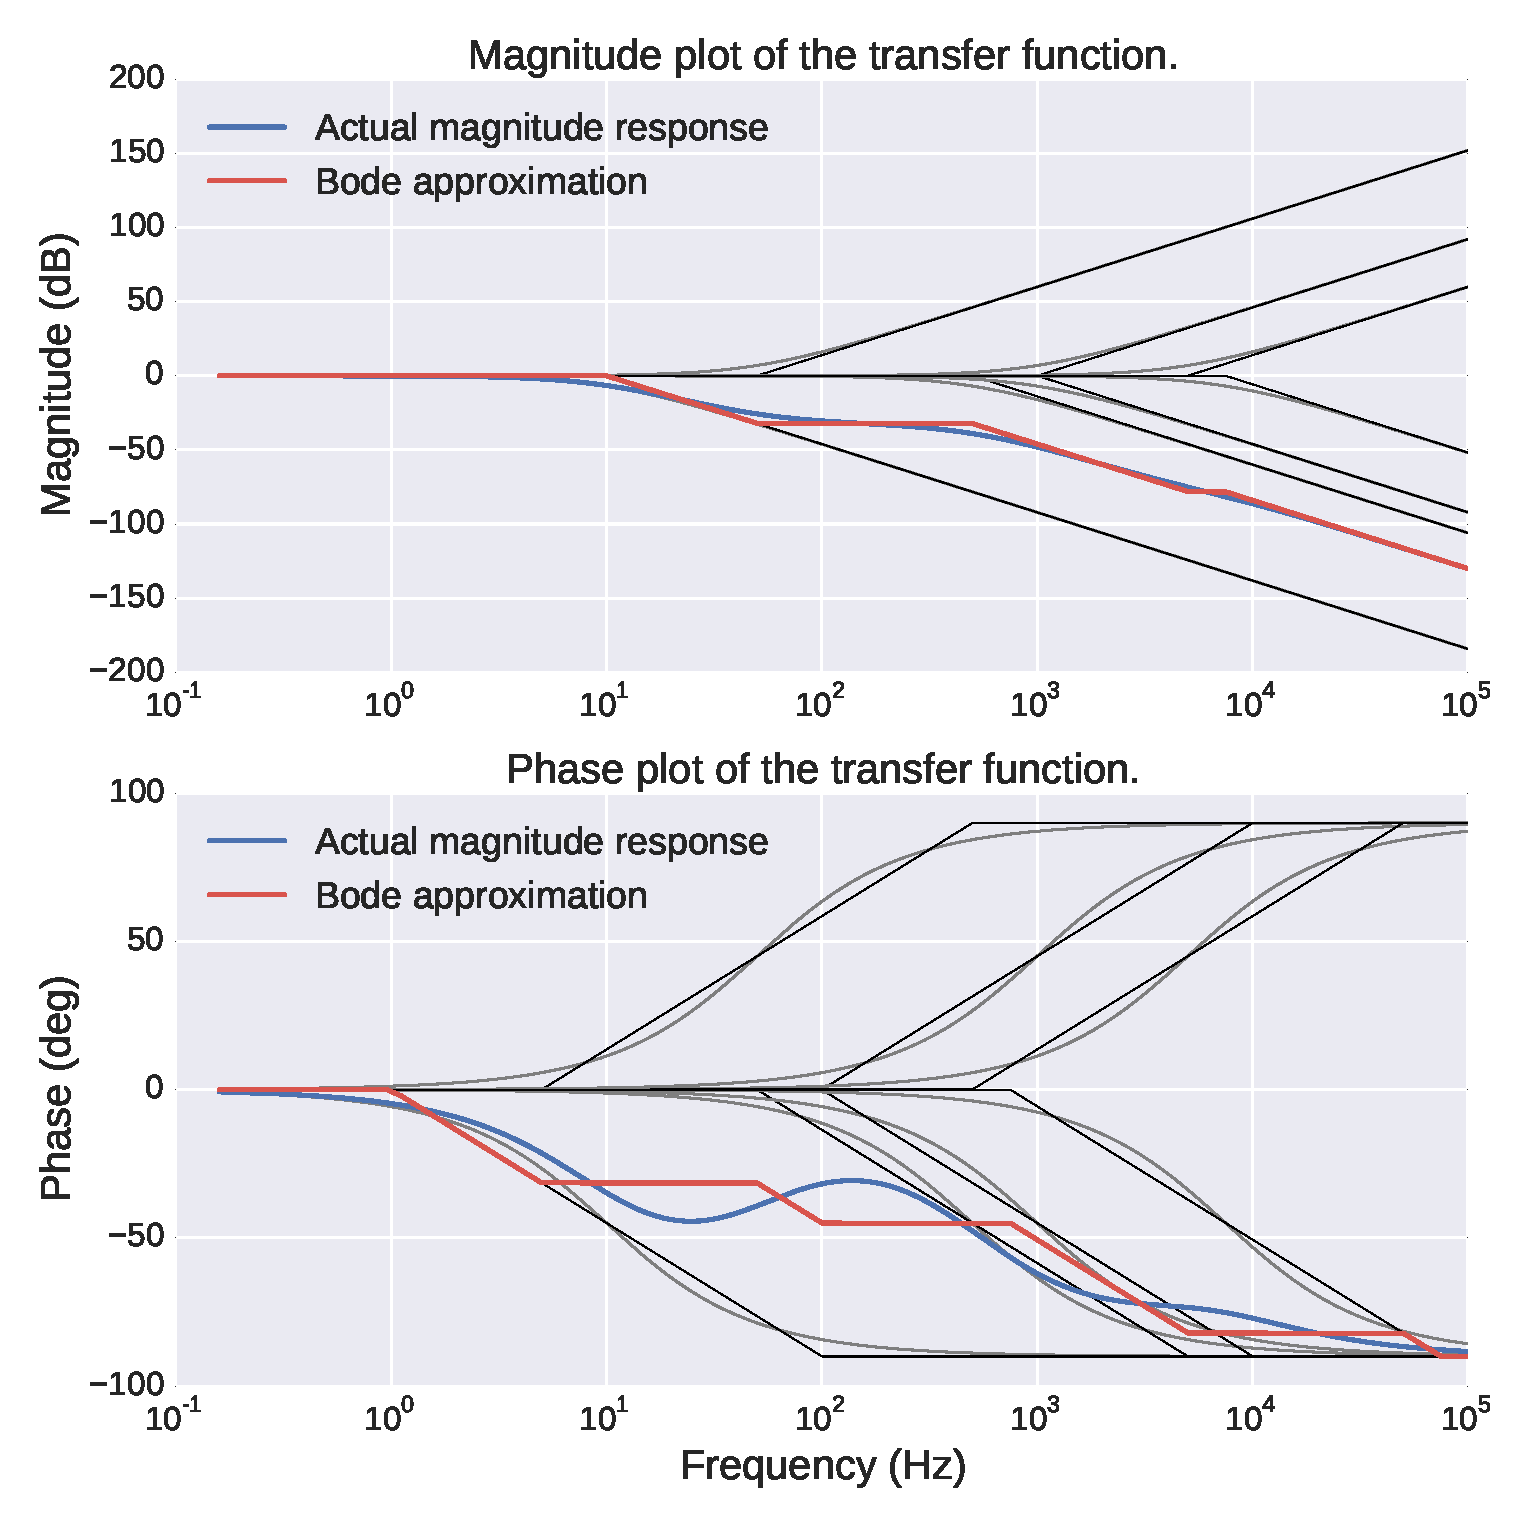
\includegraphics[width=0.6\textwidth]{img/bode.eps}
\end{figure}
\end{frame}

\end{document}